\subsection{part b}
I use a zero and a far pole to make controller feasible.

Controller:
$$
C(s) = \dfrac{2.2368\times10^5(s+11.91)}{s+10^4}
$$
Phase margin is above 40 degree.
\begin{figure}[H]
    \caption{Phase margin with controller}
    \centering
    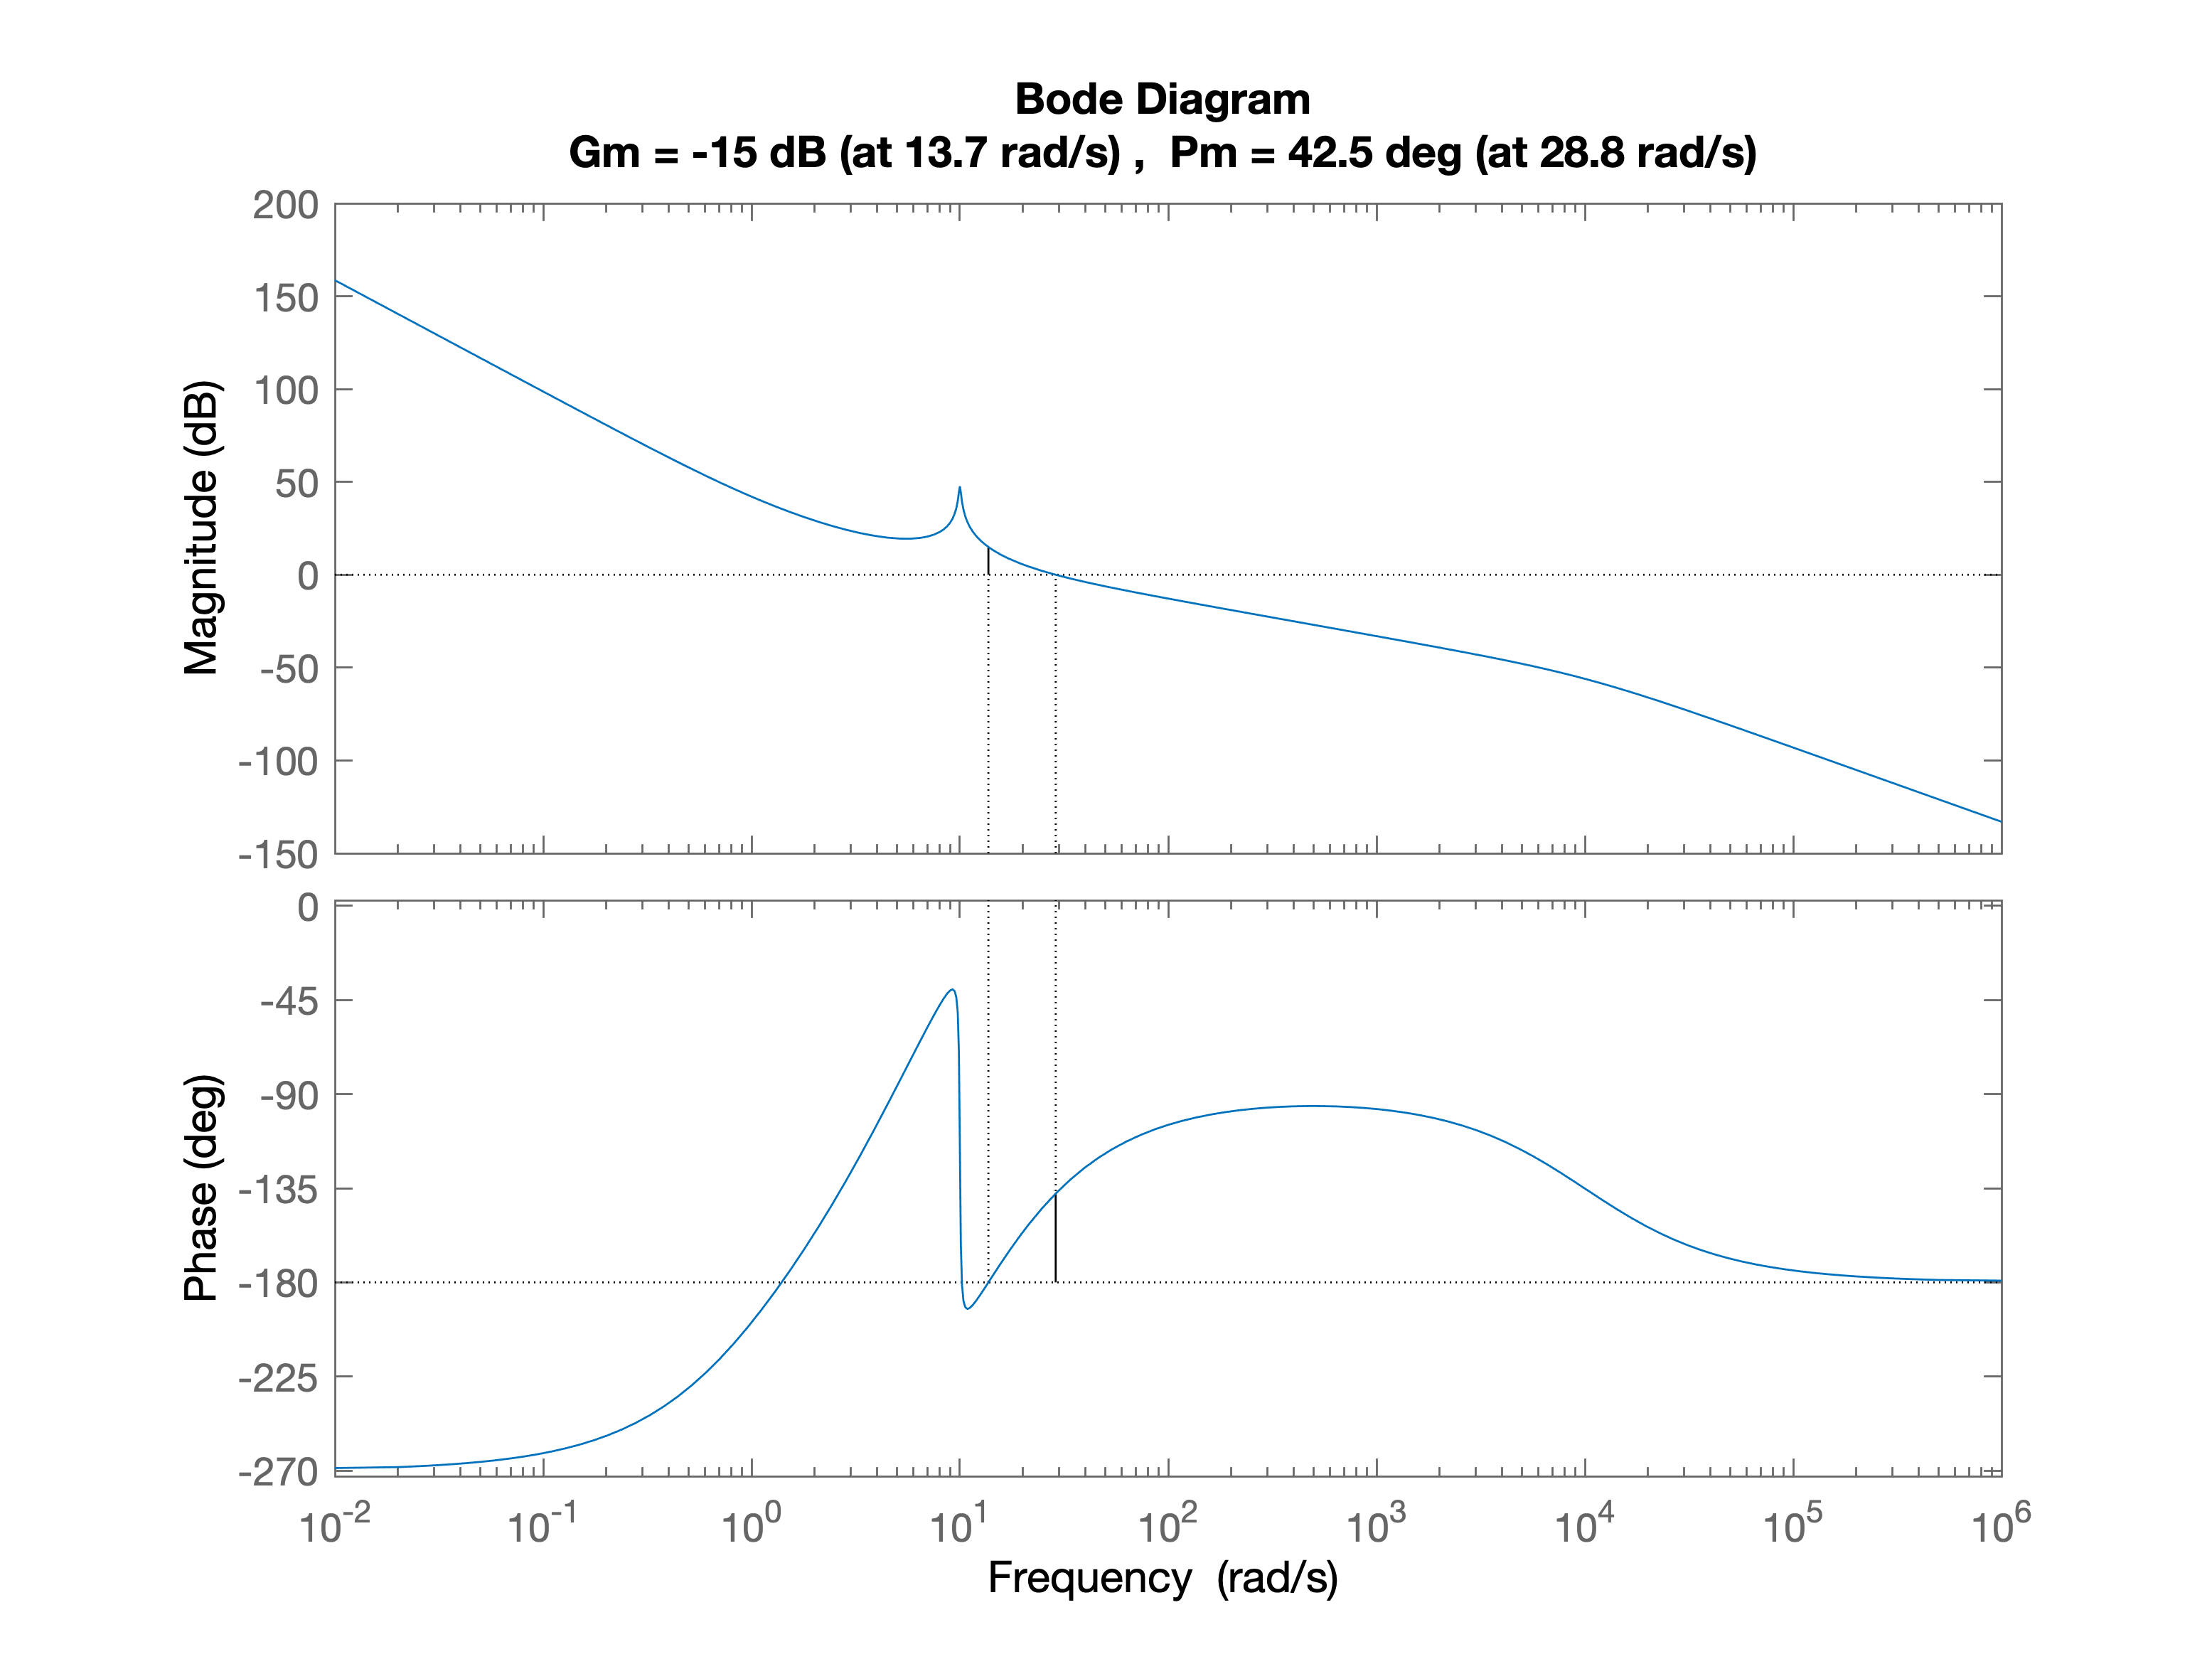
\includegraphics[width=12cm]{../Figure/Q1/Q1_b/margin.png}
\end{figure}
Maximum closed loop is below than 3 decibels.
\begin{figure}[H]
    \caption{Nichols chart with controller}
    \centering
    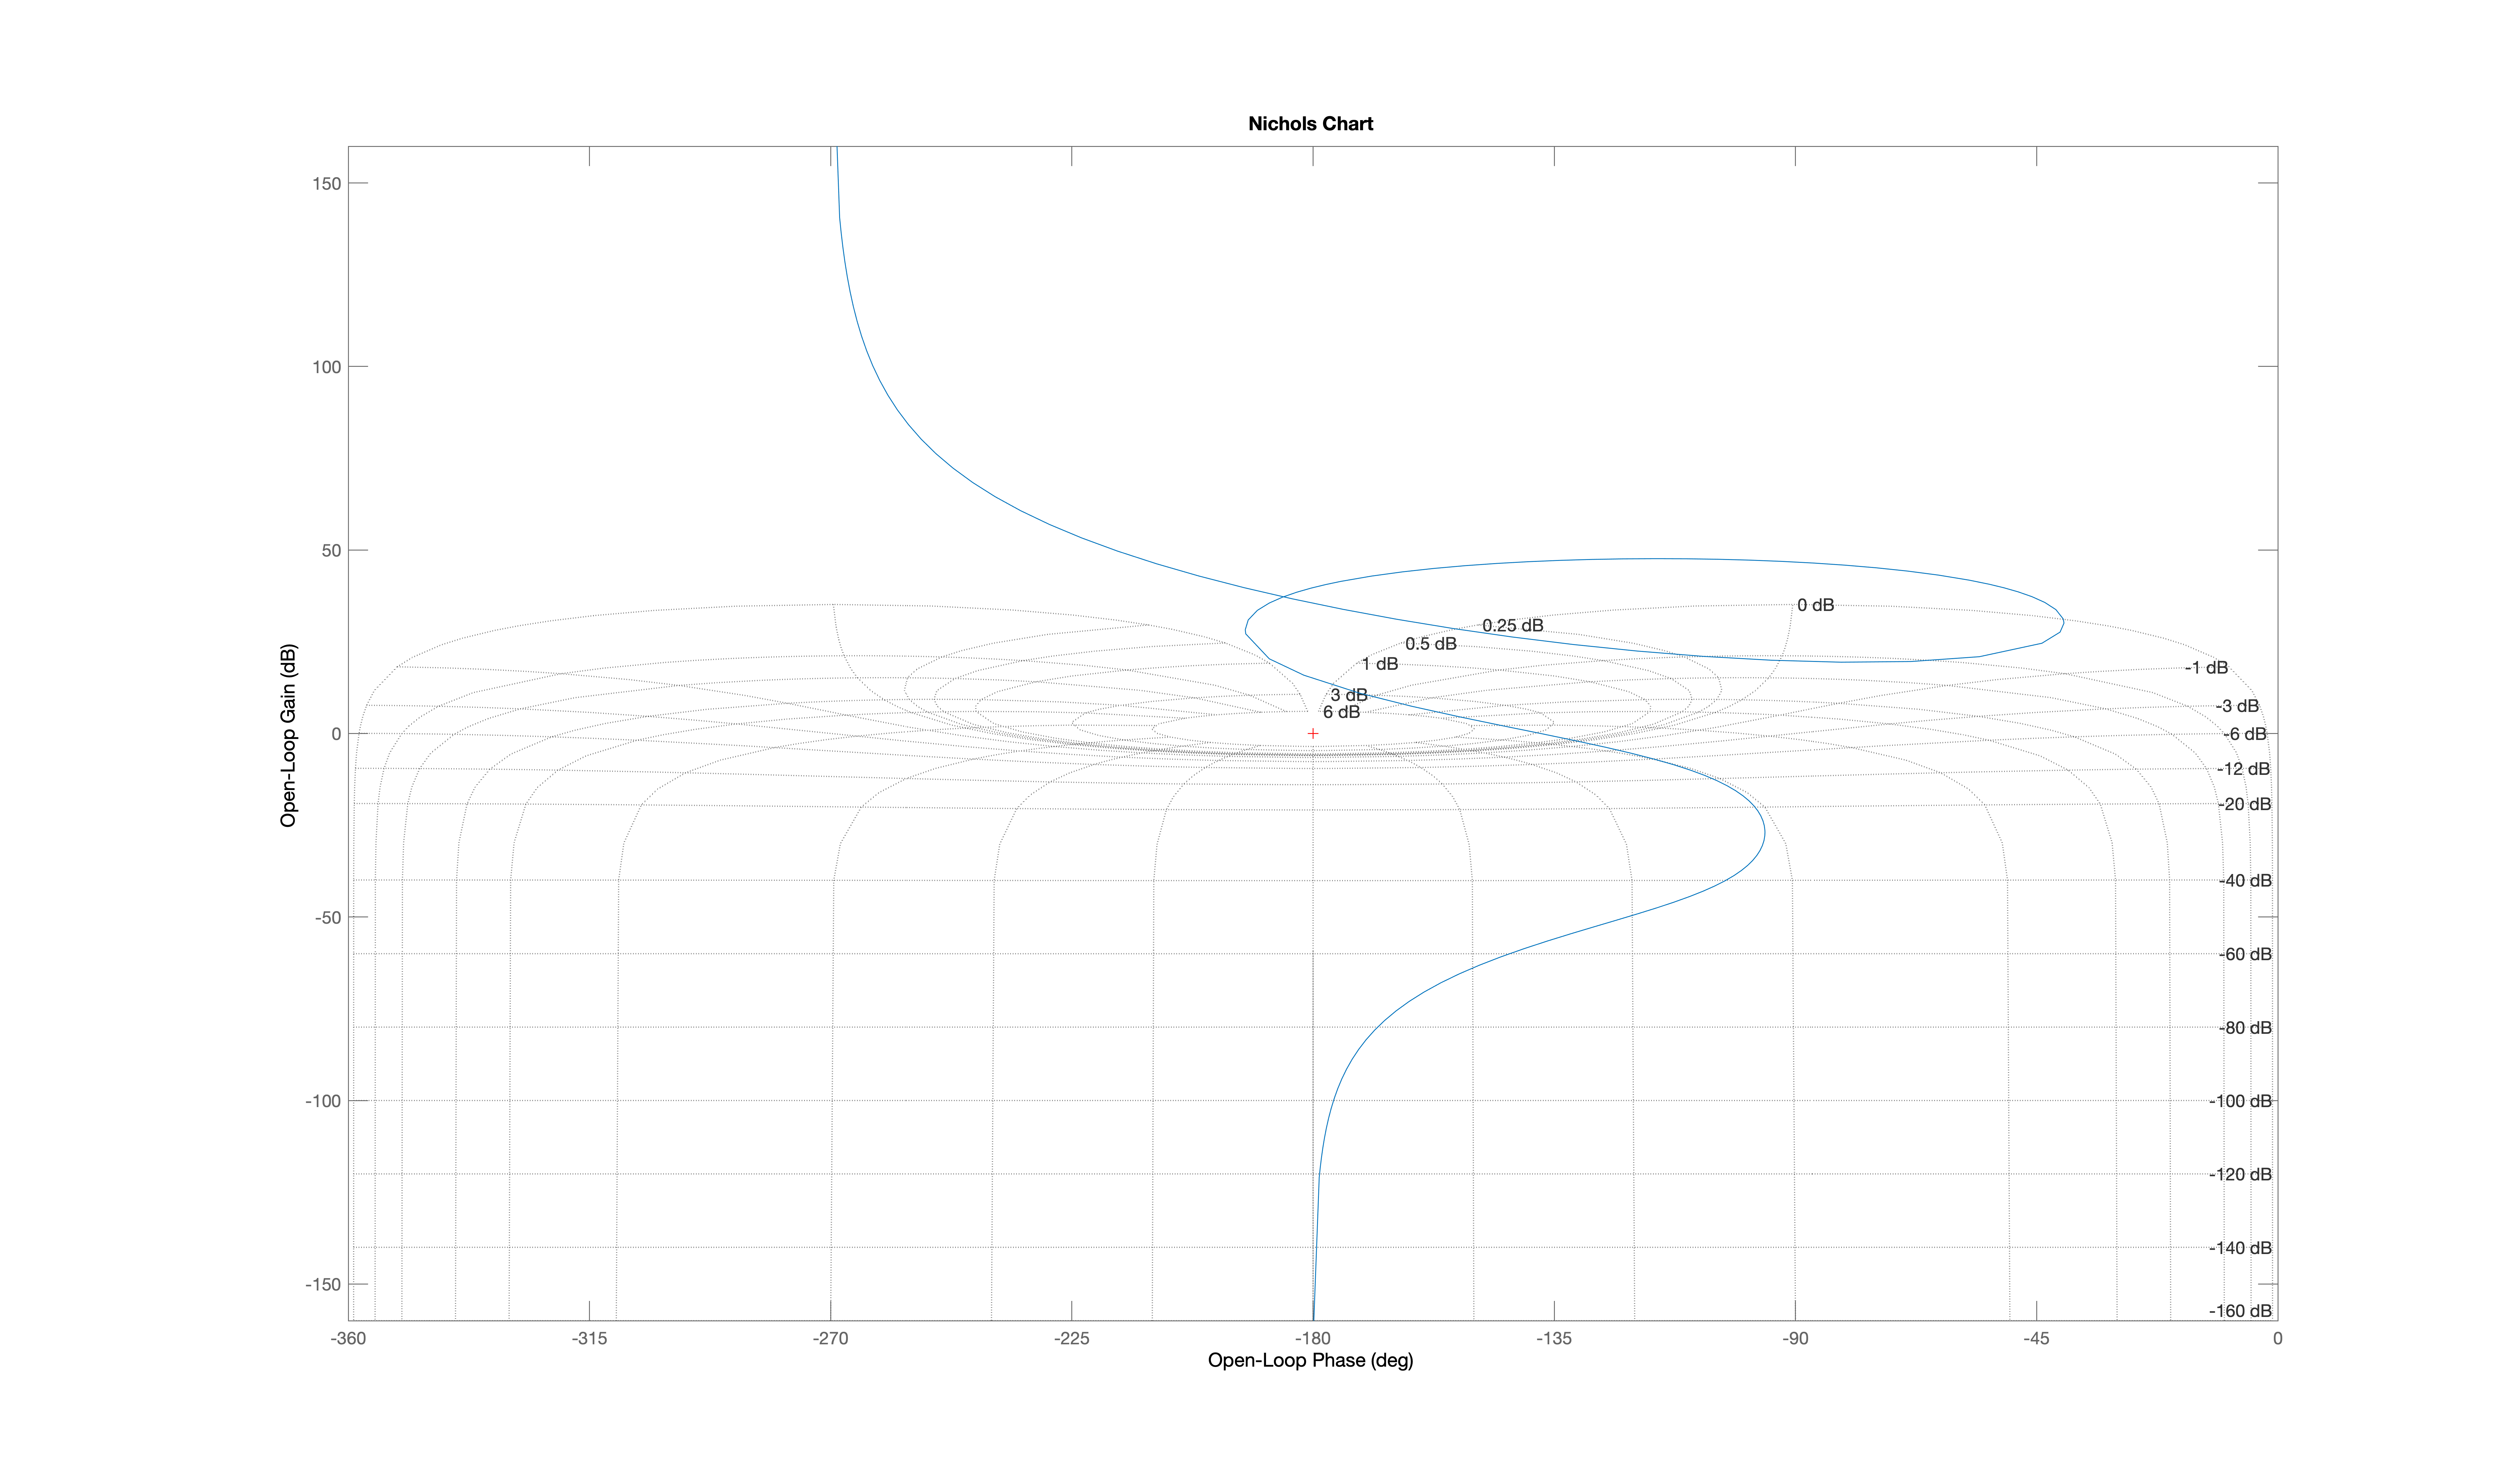
\includegraphics[width=16cm]{../Figure/Q1/Q1_b/nichols.png}
\end{figure}
Setteing time and overshoot for step responde in closed loop system are shown in figure.
\begin{figure}[H]
    \caption{Step responde}
    \centering
    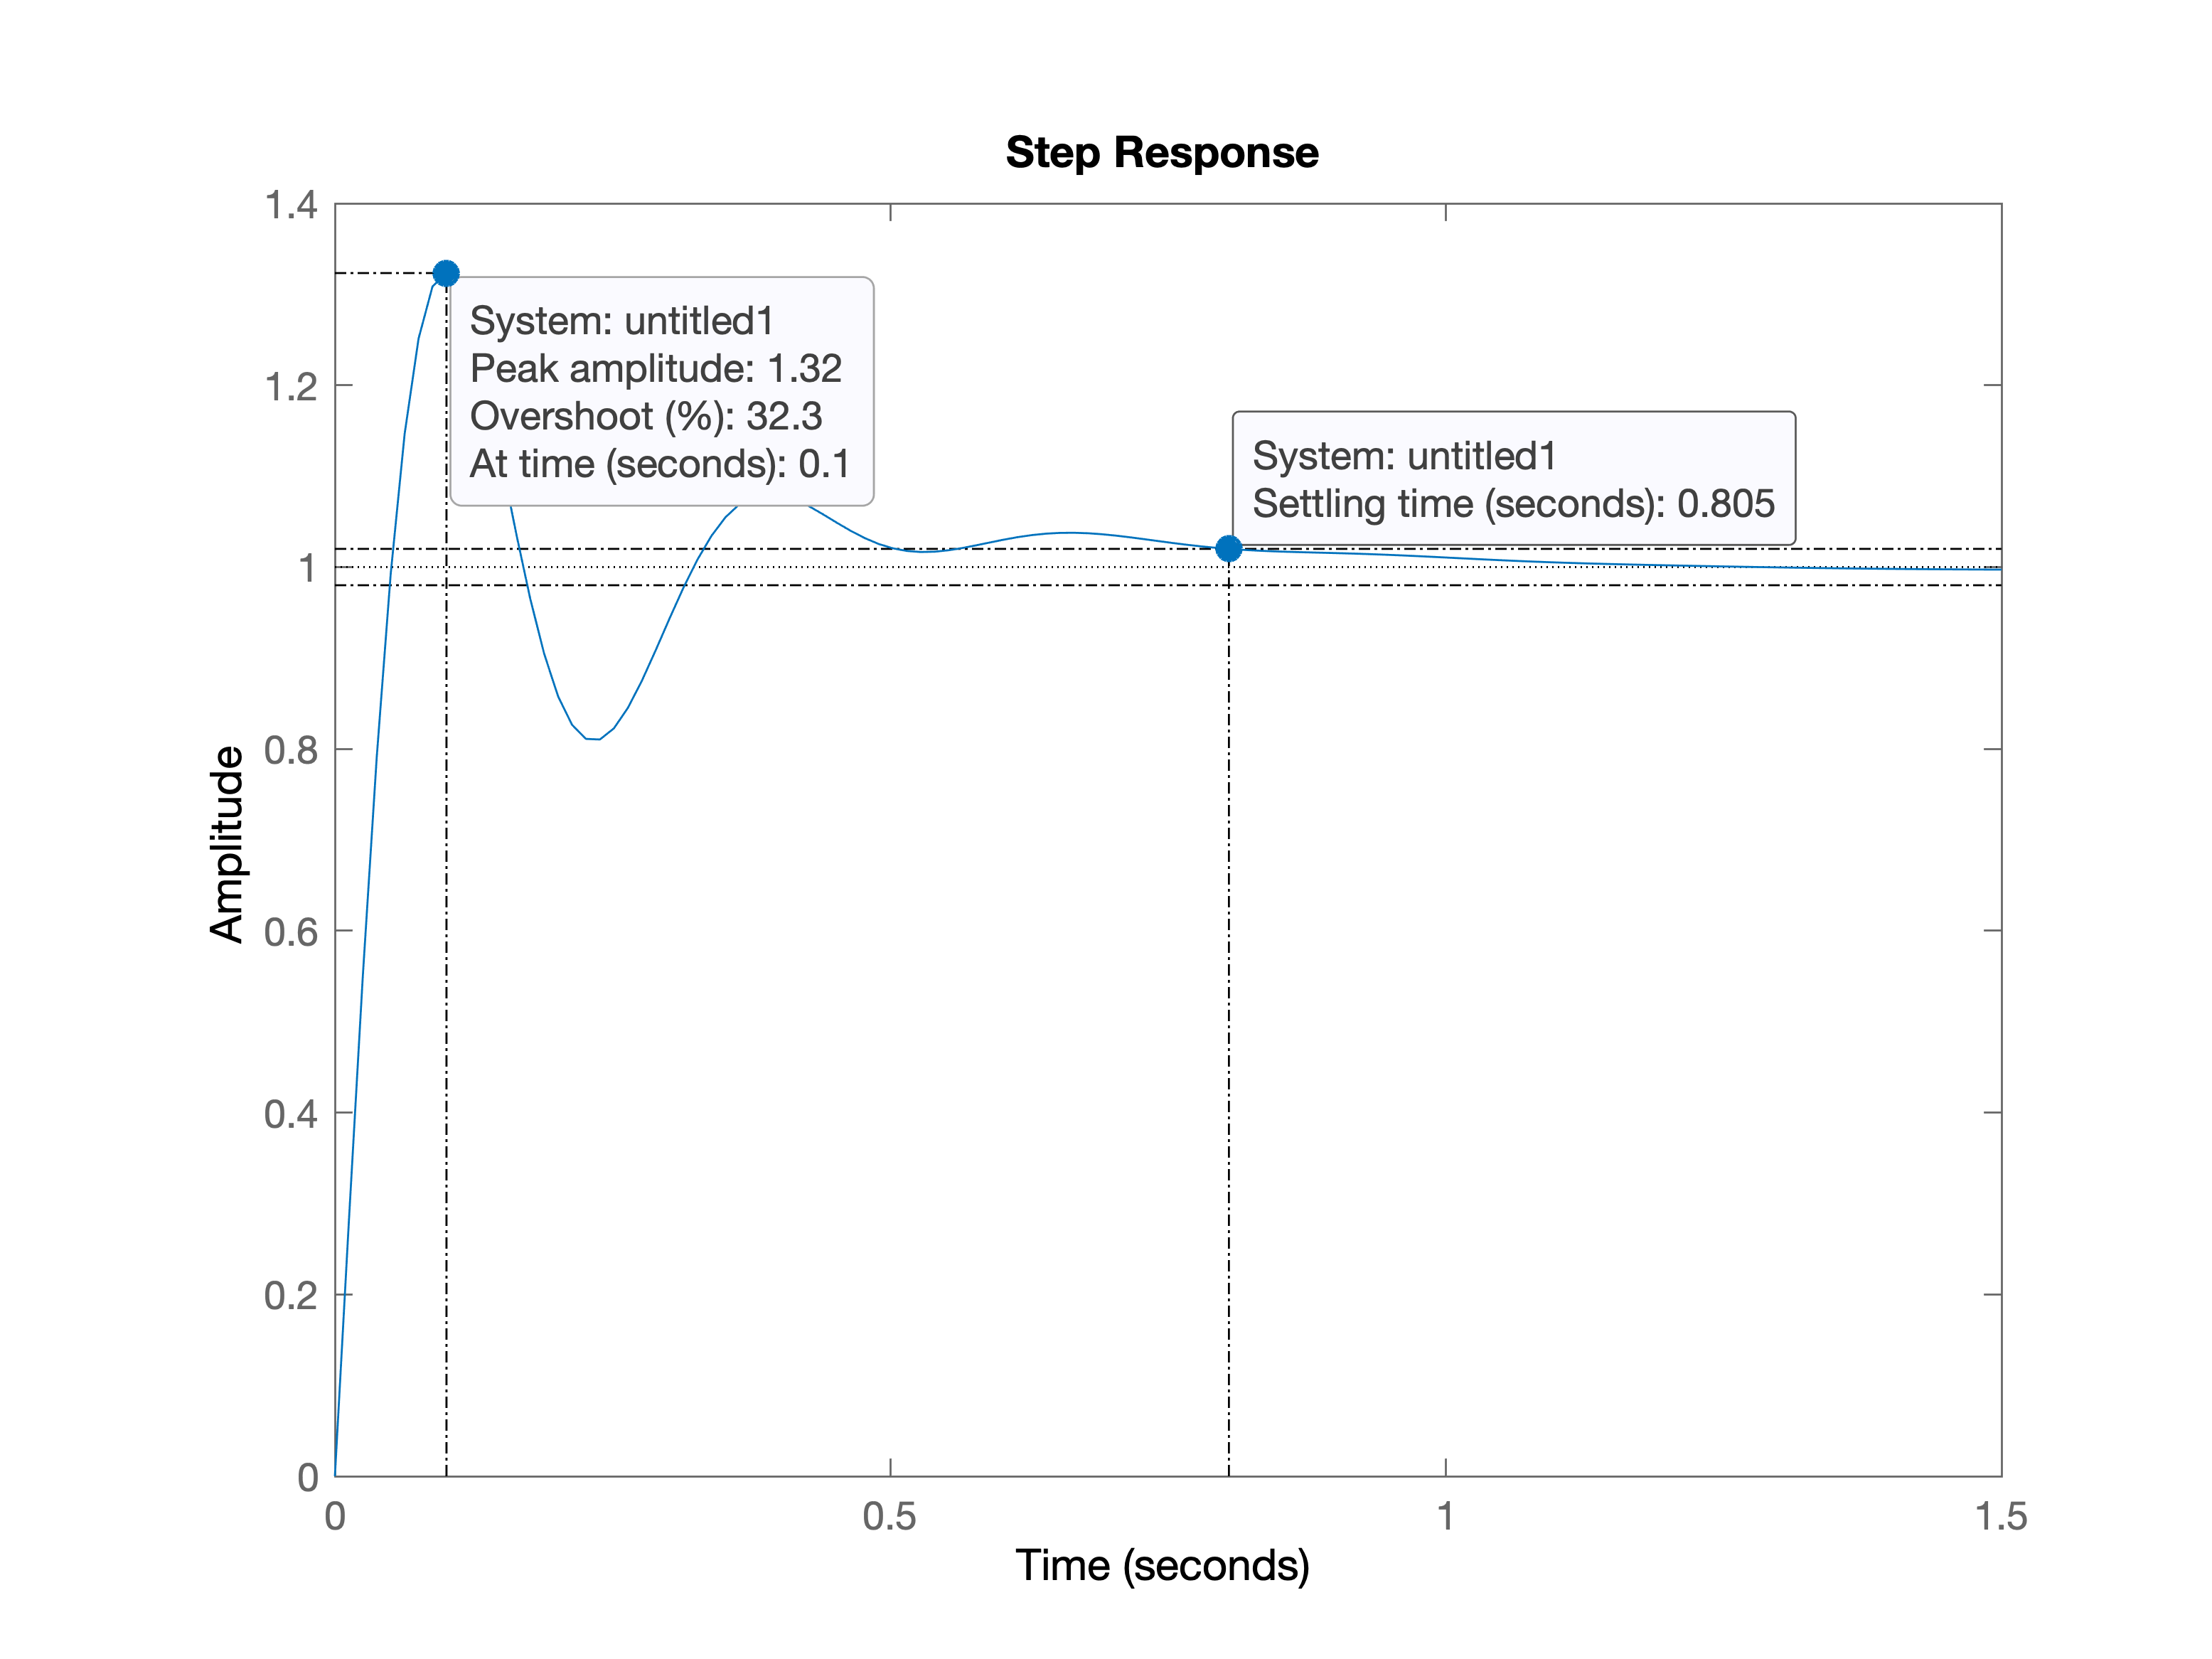
\includegraphics[width=12cm]{../Figure/Q1/Q1_b/step.png}
\end{figure}
